\documentclass[11pt,a4paper]{article}
\usepackage[a4paper,margin=2.6cm]{geometry}
\usepackage{iftex}
\ifPDFTeX
  \usepackage[T1]{fontenc}
  \usepackage[utf8]{inputenc}
  \usepackage[english]{babel}
\else
  \usepackage{fontspec}
  \usepackage{polyglossia}
  \setdefaultlanguage{english}
  \defaultfontfeatures{Ligatures=TeX}
  \setmainfont{Times New Roman}
  \setsansfont{Arial}
  \setmonofont{Courier New}
\fi
\usepackage{microtype}
\usepackage{mathtools,amssymb}
\usepackage{graphicx}
\usepackage{booktabs}
\usepackage{float}
\usepackage{caption}
\captionsetup{font=small,labelfont=bf}
\usepackage{enumitem}
\setlist{nosep,leftmargin=1.5em}
\usepackage{csquotes}
\usepackage[backend=biber,style=numeric-comp,sorting=none,maxbibnames=6]{biblatex}
\addbibresource{references_v2_en.bib}
\usepackage[unicode,hidelinks]{hyperref}
\setlength{\emergencystretch}{2em}

\title{Coupling of the hierarchical levels of the atmospheric circulation\\
as a regional invariant}
\author{Sotiriadi, N.}
\date{2026}

\begin{document}
\maketitle

\begin{abstract}
The hierarchical levels of geosystem organization are customarily identified from the spectral and fractal properties of fields; how to measure the \emph{interaction} of the identified levels, and whether the pattern of that interaction possesses the properties of an invariant of a territory, has so far remained an open question. This paper proposes a compact descriptor of such interaction --- the coupling profile of adjacent octave levels~$P$, that is, the spatial rank correlation between the activity maps of the levels of the relative-vorticity field on the 850~hPa isobaric surface. The material is the ERA5 reanalysis for 39 domains of $20^\circ\times40^\circ$ covering the principal circulation regimes; the seasons are January--March and July--September, with three periods of 2017--2024 for the twelve substantively chosen domains and the year 2024 for the twenty-seven domains of a formal lattice. The study design rests on criteria fixed in advance, on surrogate nulls, and on the confirmation of every claim on samples that took no part in obtaining it. The profile is shown to form a stable regional signature ($p=0.001$) that persists across seasons, years and ENSO phases, is not reducible to the spectral characteristics of the levels or to symmetric statistics of cross-scale coupling, and is reproduced in the independent MERRA-2 reanalysis. The decisive test is a computation on a free-running, non-assimilating model experiment of high resolution: the regional geography of the coupling is reproduced there as well ($\rho=0.71$ against an internal ceiling of the method of $0.93$), which removes the principal limitation of studies of this kind --- the impossibility of separating a property of the atmosphere from a property of the observing network. A catalogue of tested and rejected interpretations is given, including the rejected construction of a second descriptor. The applied content of the quantity has not been established on the data and models available today; we show precisely where the limitation lies.

\smallskip
\noindent\textbf{Keywords:} hierarchical organization of geosystems, invariants, scale, atmospheric circulation, reanalysis, regionalization, generalization.
\end{abstract}

\section{The problem}
\label{sec:intro}

\subsection{Invariants of the organization of a territory}

The view of geosystems as hierarchically organized entities, in which processes of different spatio-temporal levels are linked yet not reducible to one another, is among the foundations of Russian theoretical geography. In the work of Yu.~G.~Puzachenko this idea received an operational development: the spatio-temporal hierarchy of geosystems was treated from the standpoint of oscillation theory \cite{Puzachenko1986}, an apparatus was built for identifying levels of organization from the spectral and fractal properties of geographical fields \cite{Puzachenko2004}, and the search for \emph{invariants of geosystem dynamics} --- numerical characteristics of organization that are stable in time and discriminate between territories --- was posed as a research programme in its own right \cite{Puzachenko2010}. An invariant in this understanding is not a constant of nature; it is a reproducible measure of the make-up of a territory that retains its value when the state of the system changes, and is therefore suitable for comparison and regionalization.

A direct continuation of this line is the work of A.~N.~Krenke and co-authors \cite{Krenke2019}, in which the hierarchical levels of the organization of a regional mesoclimate were identified from the two-dimensional spectra of the principal components of climatic fields: a power-law model of the spectrum played the role of a background, and departures from it --- breaks of slope and subharmonic peaks --- were interpreted as manifestations of discrete levels with characteristic linear sizes. This answered the question of \emph{where} the levels of organization lie.

The next question in logical order is how to measure the \emph{relation} between the levels: to what degree the placement of the variability of one level is predetermined by its neighbour. Quantities of this kind have not previously been constructed as self-standing characteristics of a territory, nor tested for the status of invariants. The present work addresses this question for the atmospheric circulation.

\subsection{What the existing approaches do not measure}

Instruments close in spirit have developed within three traditions, and each leaves the quantity we seek outside its scope. Cascade and multifractal descriptions \cite{LovejoySchertzer2013,Lovejoy2011,Kouhen2024} characterize the distribution of intensity \emph{along} the scale continuum, but not the spatial agreement of activity maps \emph{between} particular levels. Wavelet envelopes and their statistics --- the amplitude-modulation coefficient \cite{Farge1992,Mathis2009} and the scattering covariances that systematize it \cite{Mallat2012,BrunaMallat2013,Cheng2024} --- measure the fact of a coupling between levels, but have been applied as features for classification rather than as a climatology of the make-up of a territory; the first application of such techniques to geophysical fields with the aim of discriminating regimes appeared recently and concerns the ocean \cite{Skinner2025}. Finally, the literature on atmospheric predictability \cite{Lorenz1969,Zhang2007,RotunnoSnyder2008,Judt2020,SelzCraig2023} assigns cross-scale interaction the role of a channel through which small-scale uncertainty contaminates the synoptic level, but it \emph{models} the strength of that link rather than measuring it from data.

\subsection{Objectives}

(1)~To construct, from the relative-vorticity field, a compact descriptor of inter-level organization --- the level-coupling profile~$P$. (2)~To test its status as a regional invariant: stability across seasons, years and ENSO phases; irreducibility to the spectrum and to symmetric statistics of cross-scale coupling; reproducibility in an independent reanalysis and, more significantly, in a model experiment without data assimilation. (3)~To delimit the range of valid application, including a catalogue of tested and rejected interpretations.

\section{Material and method}
\label{sec:data}

\subsection{Data}

The principal material is the ERA5 reanalysis \cite{Hersbach2020,Soci2024}: wind components on the 850~hPa surface, $0.25^\circ$ grid, 6-hour step. The choice of the 850~hPa level reflects its representativeness for the lower-tropospheric circulation that interacts directly with the underlying surface.

The analysis is carried out in 39 domains of $20^\circ$ latitude $\times\ 40^\circ$ longitude. Twelve of them were chosen substantively and cover six contrasting circulation regimes: tropical oceans, the extratropical storm tracks of both hemispheres, centres of deep convection over land, and continental regions of the temperate and subtropical belts. The remaining 27 are set by a formal rule --- a regular lattice of $20^\circ\times40^\circ$ cells with the exclusion of those overlapping the first twelve by more than 20\,\% of area --- so that the composition of the sample cannot be suspected of tuning. The time windows are January--March and July--September. For the twelve substantively chosen domains three periods are used --- 2017--2019, 2021--2022 and 2023--2024; they correspond to opposite ENSO phases, which makes it possible to test the stability of the descriptor not only against the change of season and year but also against the change of the large-scale climatic state. The twenty-seven lattice domains, which serve to test the geography on an independent sample composition, are taken for 2024.

Two sources are enlisted for the independent test of reproducibility. The first is the MERRA-2 reanalysis \cite{Gelaro2017}, built on a different general-circulation model and a different assimilation system. The second, fundamentally stronger one, is the \texttt{highresSST-present} experiment of the HighResMIP project \cite{Haarsma2016} with the ECMWF-IFS-HR model \cite{Roberts2018}: an integration with prescribed sea-surface temperature that \emph{assimilates no atmospheric observations whatsoever}. Comparison with it answers the question that a comparison of two reanalyses cannot resolve in principle: whether the measured property belongs to the atmosphere or to the geography of the observing network \cite{BonavitaLaloyaux2020}.

A limitation of the material is stated in advance: the effective resolution of modern reanalyses is 4--7 grid steps \cite{Skamarock2004,Bolgiani2022}, that is, about 150--200~km for ERA5. Variability on smaller scales is shaped to a considerable degree by numerical dissipation and parameterizations rather than by resolved dynamics; all principal conclusions are therefore duplicated by a control restricted to the ``resolved'' levels coarser than 200~km, and comparison with external sources is conducted on those levels only.

\subsection{Levels and activity maps}

The working field is the relative vorticity $\omega$, computed with the metric of the sphere taken into account. Vorticity is preferable to the wind components in that it emphasizes the rotational structure of the flow and suppresses the large-scale advective background.

The decomposition into levels is built by successive Gaussian smoothing with the set of scales $\ell\in\{50,100,200,400,800,1600\}$~km. Level~$i$ is defined as the difference of adjacent smoothings,
\begin{equation}
D_i(x,y,t)=\overline{\omega}_{\ell_i}-\overline{\omega}_{\ell_{i+1}},
\end{equation}
and contains structures with characteristic sizes between $\ell_i$ and $\ell_{i+1}$ (an octave). This decomposition corresponds directly to the identification of levels of organization from the spectrum \cite{Krenke2019}, but transfers the analysis from spectral space to physical space: for each level an \emph{activity map} (envelope)
\begin{equation}
E_i(x,y,t)=\overline{\lvert D_i\rvert}_{\ell_{i+1}}
\end{equation}
is built, showing \emph{where} the variability of that level is concentrated at a given moment. The use of envelopes as indicators of the local activity of a scale goes back to the wavelet analysis of turbulence \cite{Farge1992}. All spatial statistics are computed over the interior of a domain, with a boundary strip excluded.

\subsection{The descriptor}

The level-coupling profile $P=(\rho_1,\dots,\rho_5)$ is the spatial rank correlation of the logarithms of the activity maps of adjacent levels:
\begin{equation}
\rho_i(t)=\operatorname{corr}_{\mathrm{rank}}\!\left[\ln E_{i-1}(\cdot,t),\ \ln E_{i}(\cdot,t)\right],
\label{eq:rho}
\end{equation}
followed by the median over the time steps of a seasonal window. In substance, $\rho_i$ answers the question of whether the structures of the finer level are active in the same places as the structures of the adjacent coarse one --- that is, how far the placement of variability on one floor of the hierarchy is predetermined by its neighbour. The rank form of the correlation makes the descriptor insensitive to any monotone transformation of amplitude and, in particular, to regional differences in the overall intensity of the circulation. This is essential: as shown below, it is precisely insensitivity to amplitude that separates a workable construction from an unworkable one.

One methodological circumstance is important. The overlap of adjacent Gaussian octaves by itself produces a non-zero coupling even for a random field with the same spectrum. Alongside the raw profile we therefore consider the \emph{excess over a surrogate}, $P-P_{\mathrm{surr}}$, where $P_{\mathrm{surr}}$ is the median profile of an ensemble of fields with the spatial spectrum preserved and the phases randomized. This excess is free of the filter-overlap contribution and reflects the properly non-Gaussian organization of the field.

\subsection{Design of the testing}

The study follows a falsification scheme. The criteria of every stage were fixed \emph{before} the corresponding data were consulted, all deviations were logged, and every key claim was confirmed on samples that took no part in obtaining it. The stability of the signatures was assessed by permutation clustering tests: for the standardized descriptors, the median Euclidean distances ``within a region'' and ``between regions'' were compared, with significance determined over 999 permutations of the regional labels. Irreducibility to simpler characteristics was tested by leave-one-out residualization: the part of the descriptor linearly predictable from a control feature set was removed, and the clustering test was repeated. The control sets were, in turn, spectral features; the semi-fractal characteristics of the levels --- direct analogues of the features by which the levels are identified in \cite{Krenke2019}; second-order scattering statistics \cite{Cheng2024}; and the geometric characteristics of the domains.

\section{Results}
\label{sec:results}

\subsection{The geography of coupling}

The coupling profile decreases monotonically from the fine levels to the coarse ones in all domains, but the rate of decrease, and the level at which the main loss of coupling occurs, differ regionally and stably (Fig.~\ref{fig:profiles}). The value of the profile on the resolved steps ranges from 0.51 to 0.73 (Fig.~\ref{fig:pmap}).

The geography reads meaningfully. The greatest coupling belongs to the extratropical storm tracks: the frontal structure manifests itself coherently on all levels, and from the large-scale field one can point to where the mesoscale will be located. The smallest belongs to the moist-convective oceanic regimes, where mesoscale organization is generated by processes weakly determined by the large-scale field. The continental regions of the temperate belt occupy an intermediate position.

\begin{figure}[t]
\centering
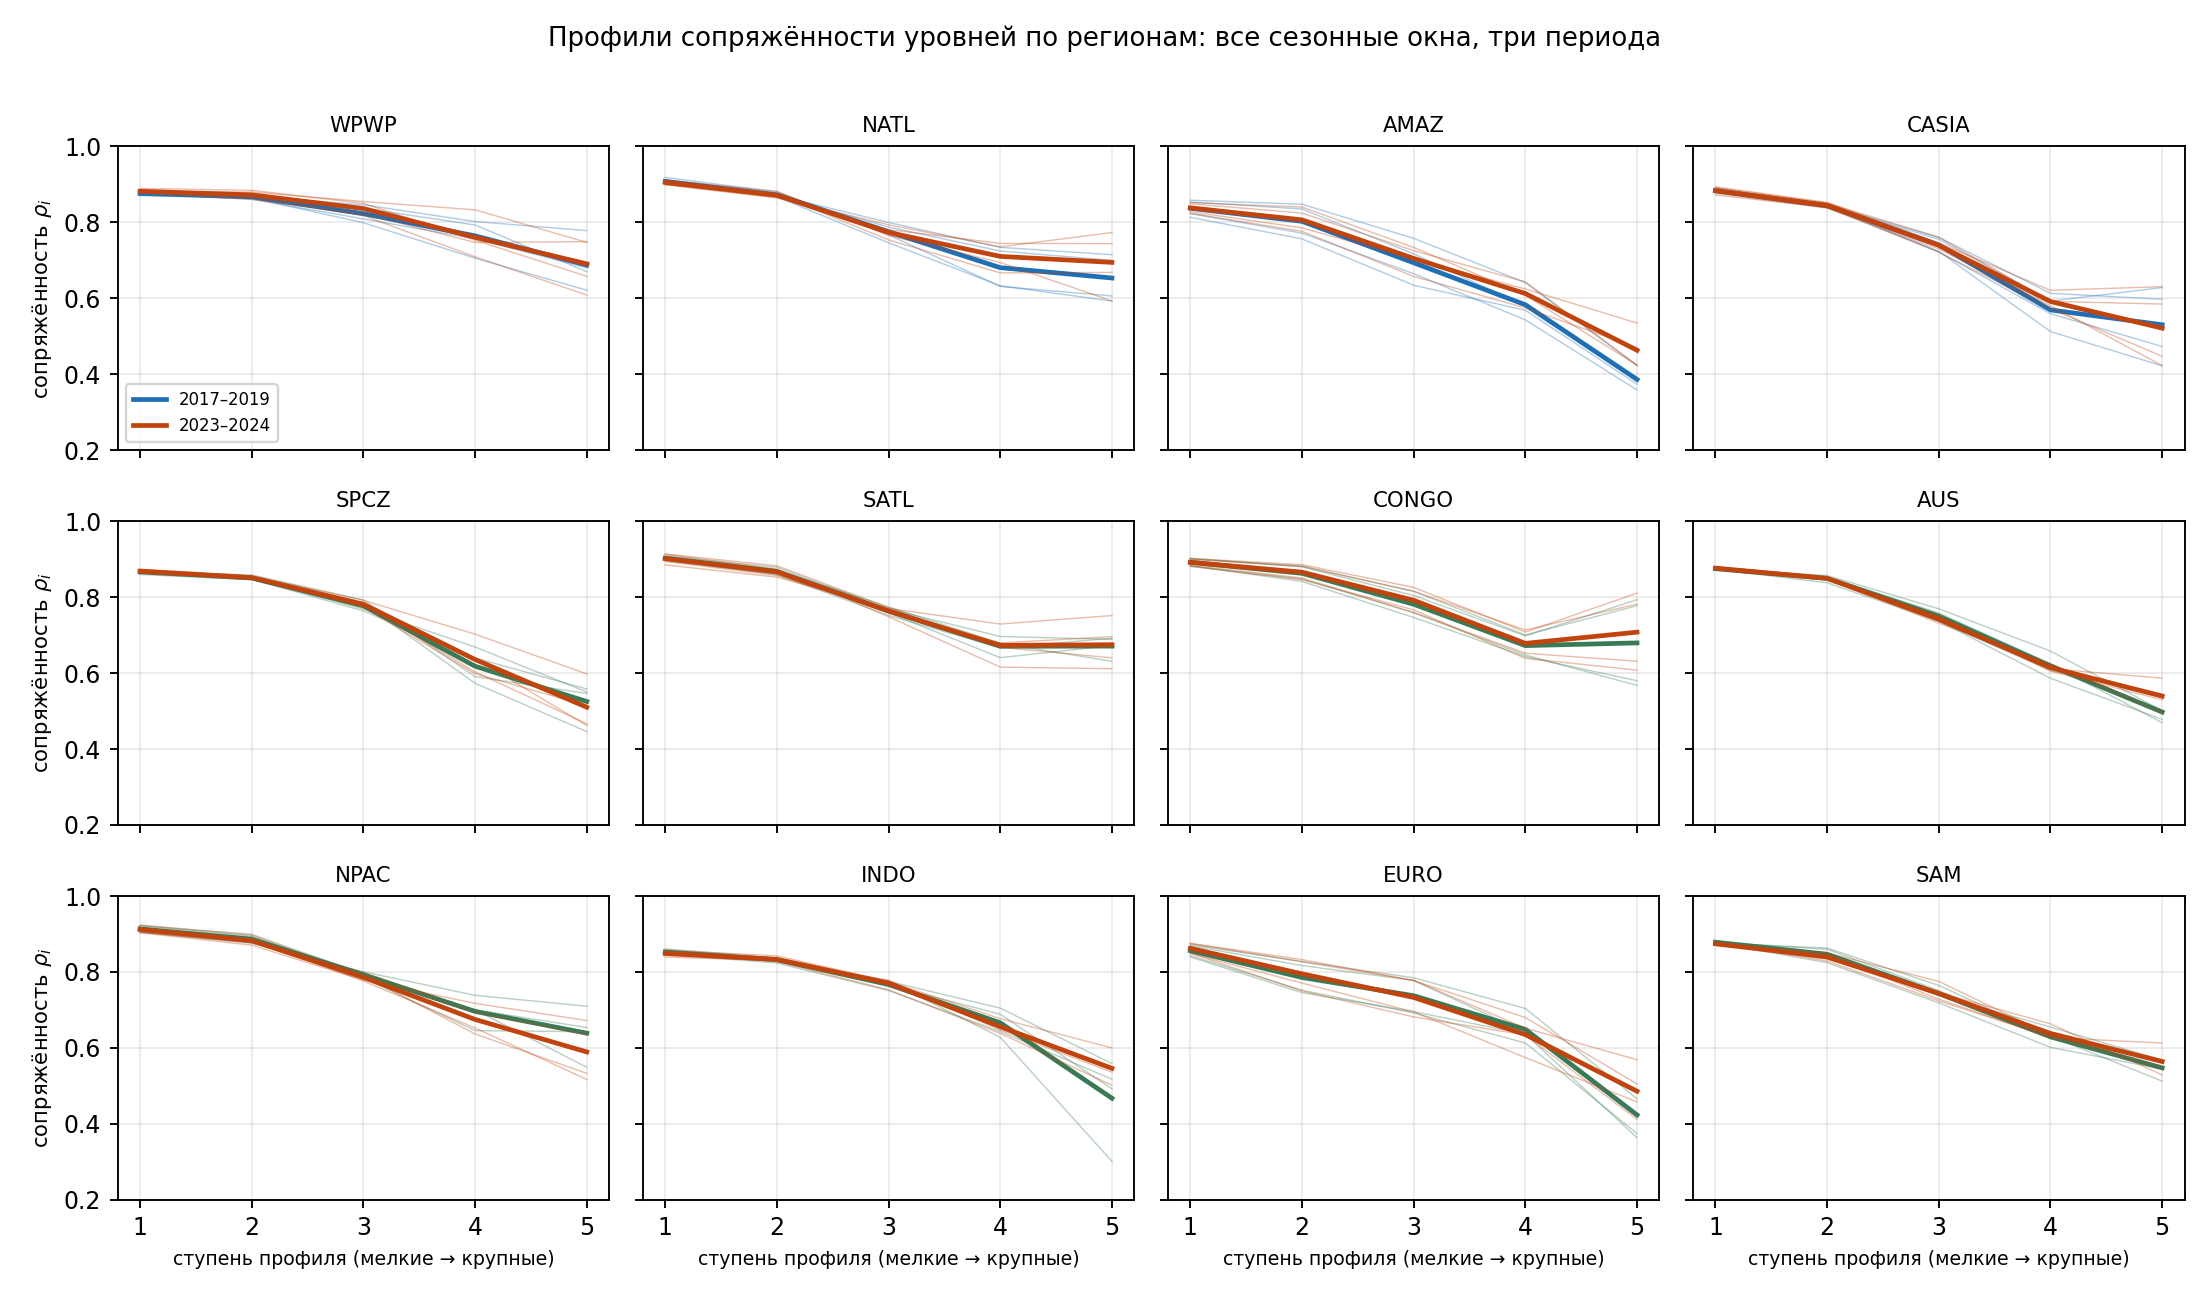
\includegraphics[width=\linewidth]{figures/figP_profiles.png}
\caption{Level-coupling profiles $P$: thin lines --- individual seasonal windows, thick lines --- averages over the periods 2017--2019, 2021--2022 and 2023--2024. Steps 1--5 correspond to pairs of adjacent levels: from (finer than 50; 50--100~km) to (400--800; 800--1600~km). Panel labels are in Russian in this release.}
\label{fig:profiles}
\end{figure}

\begin{figure}[t]
\centering
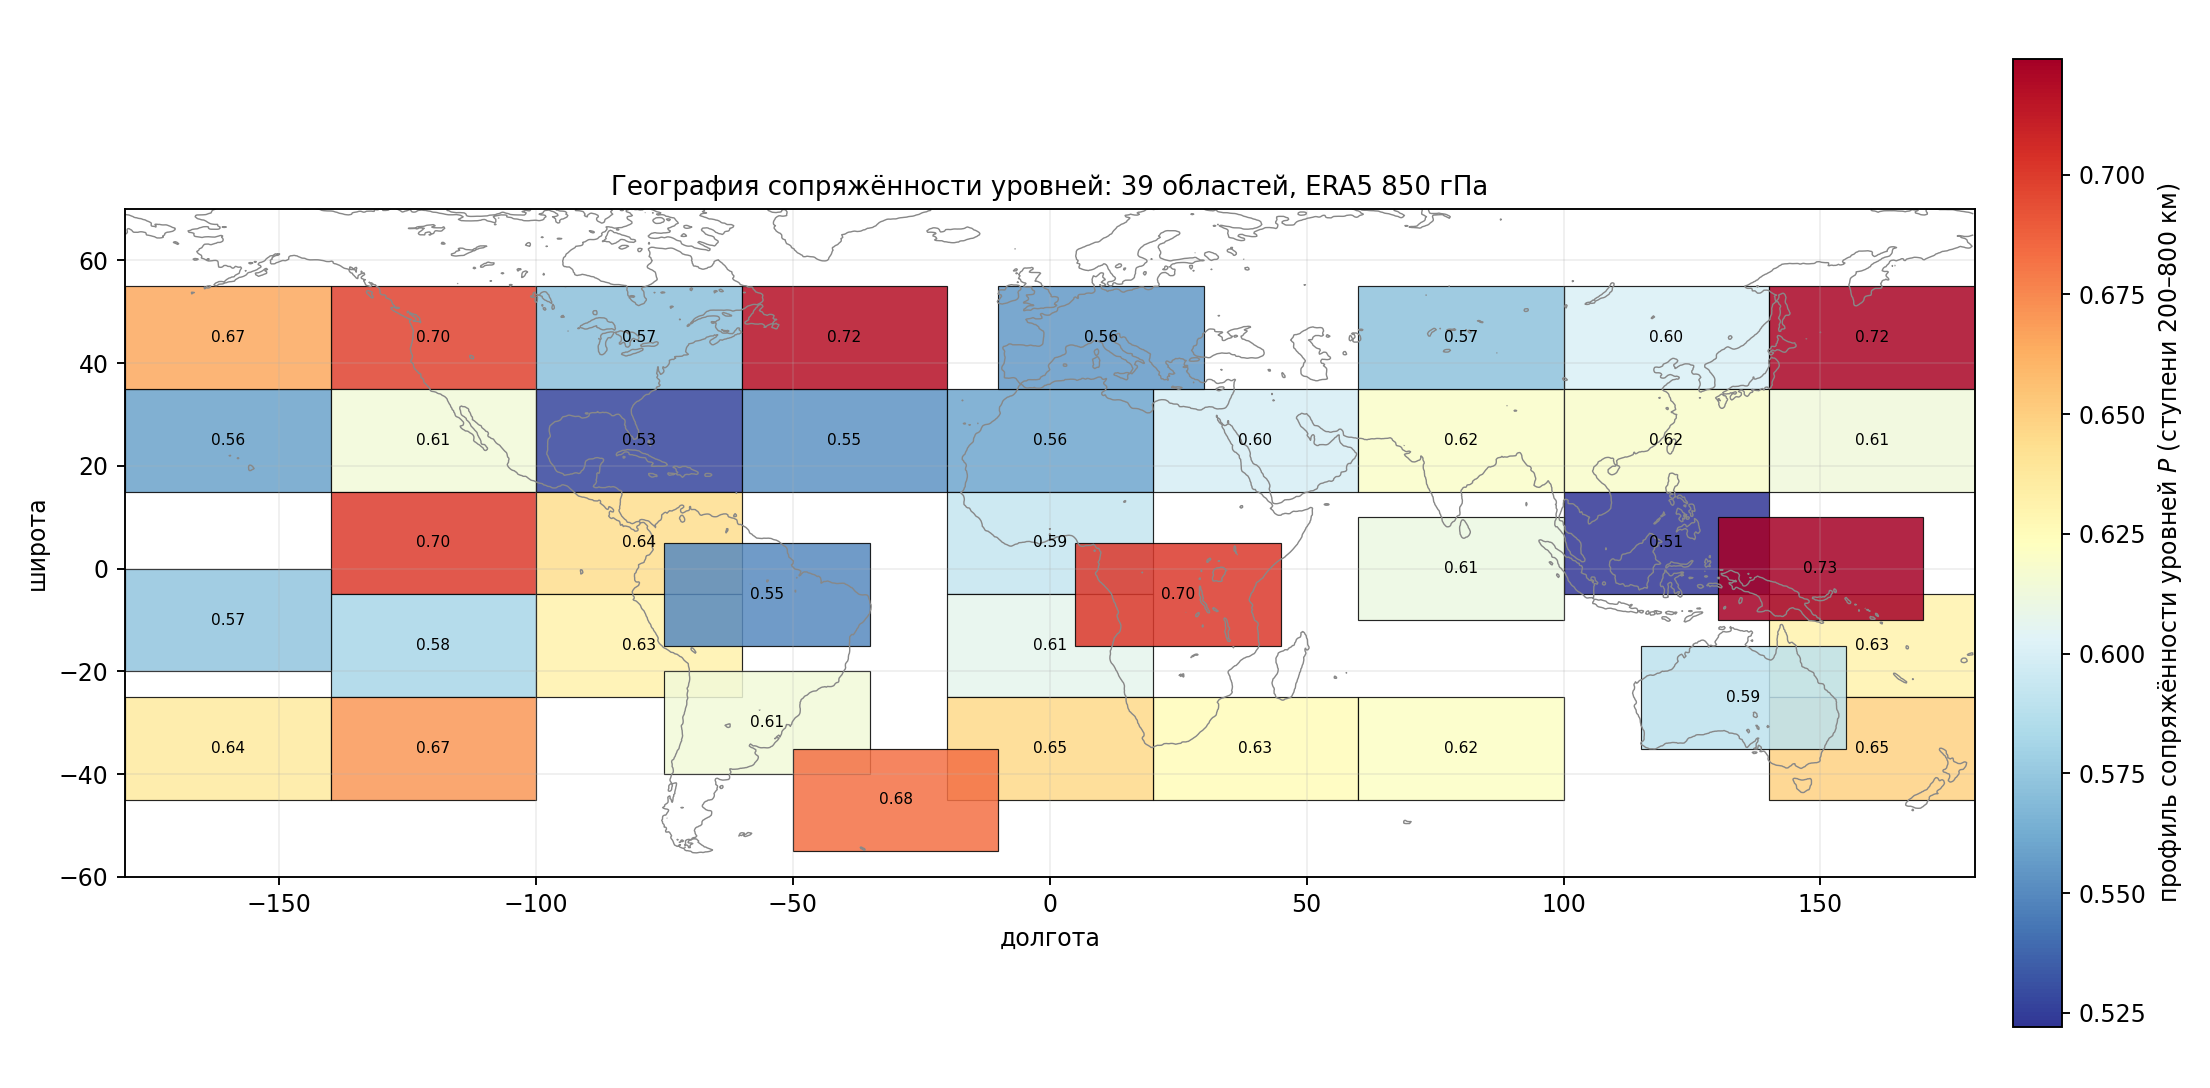
\includegraphics[width=\linewidth]{figures/figP_world_map.png}
\caption{The geography of level coupling: profile values on the resolved steps (200--800~km) for the 39 domains, ERA5, 850~hPa. Twelve domains were chosen substantively, 27 by the formal lattice rule.}
\label{fig:pmap}
\end{figure}

\subsection{What survives the controls}

The results of the tests are collected in Table~\ref{tab:tests}. The profile forms a stable regional signature on samples that took no part in its construction, is not reducible to the semi-fractal characteristics of the levels or to the scattering statistics, and is reproduced in an independent reanalysis. One reservation is stated explicitly: the independence of the profile from the full power spectrum is conditional --- it is confirmed under the control of spectral features but does not survive the additional control of domain geometry ($p=0.10$). In other words, part of the inter-regional differences of the profile is connected with the latitude of a domain and the grid spacing, and we do not claim complete irreducibility to the spectrum.

\begin{table}[t]
\centering
\caption{Summary of the tests of the coupling profile. Significance levels of the permutation clustering tests are given (999 permutations of regional labels); ``independent years'' are samples that took no part in the construction of the descriptor.}
\label{tab:tests}
\small
\begin{tabular}{@{}p{0.62\linewidth}p{0.30\linewidth}@{}}
\toprule
Test & Outcome\\
\midrule
Regional signature, independent years and ENSO phases & $p=0.001$\\
Beyond the semi-fractal level characteristics \cite{Krenke2019} & $p=0.001$\\
Beyond the scattering statistics \cite{Cheng2024} & $p=0.026$\\
Beyond the full power spectrum & $p=0.029$; with the geometry control $p=0.10$\\
Resolved levels only (from 200~km) & $p=0.002$\\
Signature in MERRA-2 & $p=0.001$\\
Agreement with the computation on a non-assimilating model & $\rho=0.71$; $p=0.001$\\
\bottomrule
\end{tabular}
\end{table}

\subsection{The test on a computation without data assimilation}

Agreement between two reanalyses is insufficient for a claim about a property of the atmosphere: ERA5 and MERRA-2 assimilate largely the same observations, and the coincidence of their geographies may reflect the geography of the observing network \cite{BonavitaLaloyaux2020}. The decisive test is a computation on a free-running model that assimilates no observations at all.

Such a comparison has been performed (Fig.~\ref{fig:free}). The regional geography of coupling in the \texttt{highresSST-present} experiment reproduces the ERA5 geography with a rank correlation of $\rho=0.71$ ($p=0.001$, 39 domains). This figure should be judged against the internal ceiling of the method: the correlation between two independent periods of ERA5 itself is $0.93$, so about three quarters of what is attainable has been attained. The difference is natural: a free-running integration reproduces the climatology of the regimes, not their particular realization.

The conclusion matters for the whole enterprise: the measured property belongs to the atmosphere, not to the observing system and not to the assimilation system. The limitation that in studies of this kind usually remains insurmountable is here removed.

\begin{figure}[t]
\centering
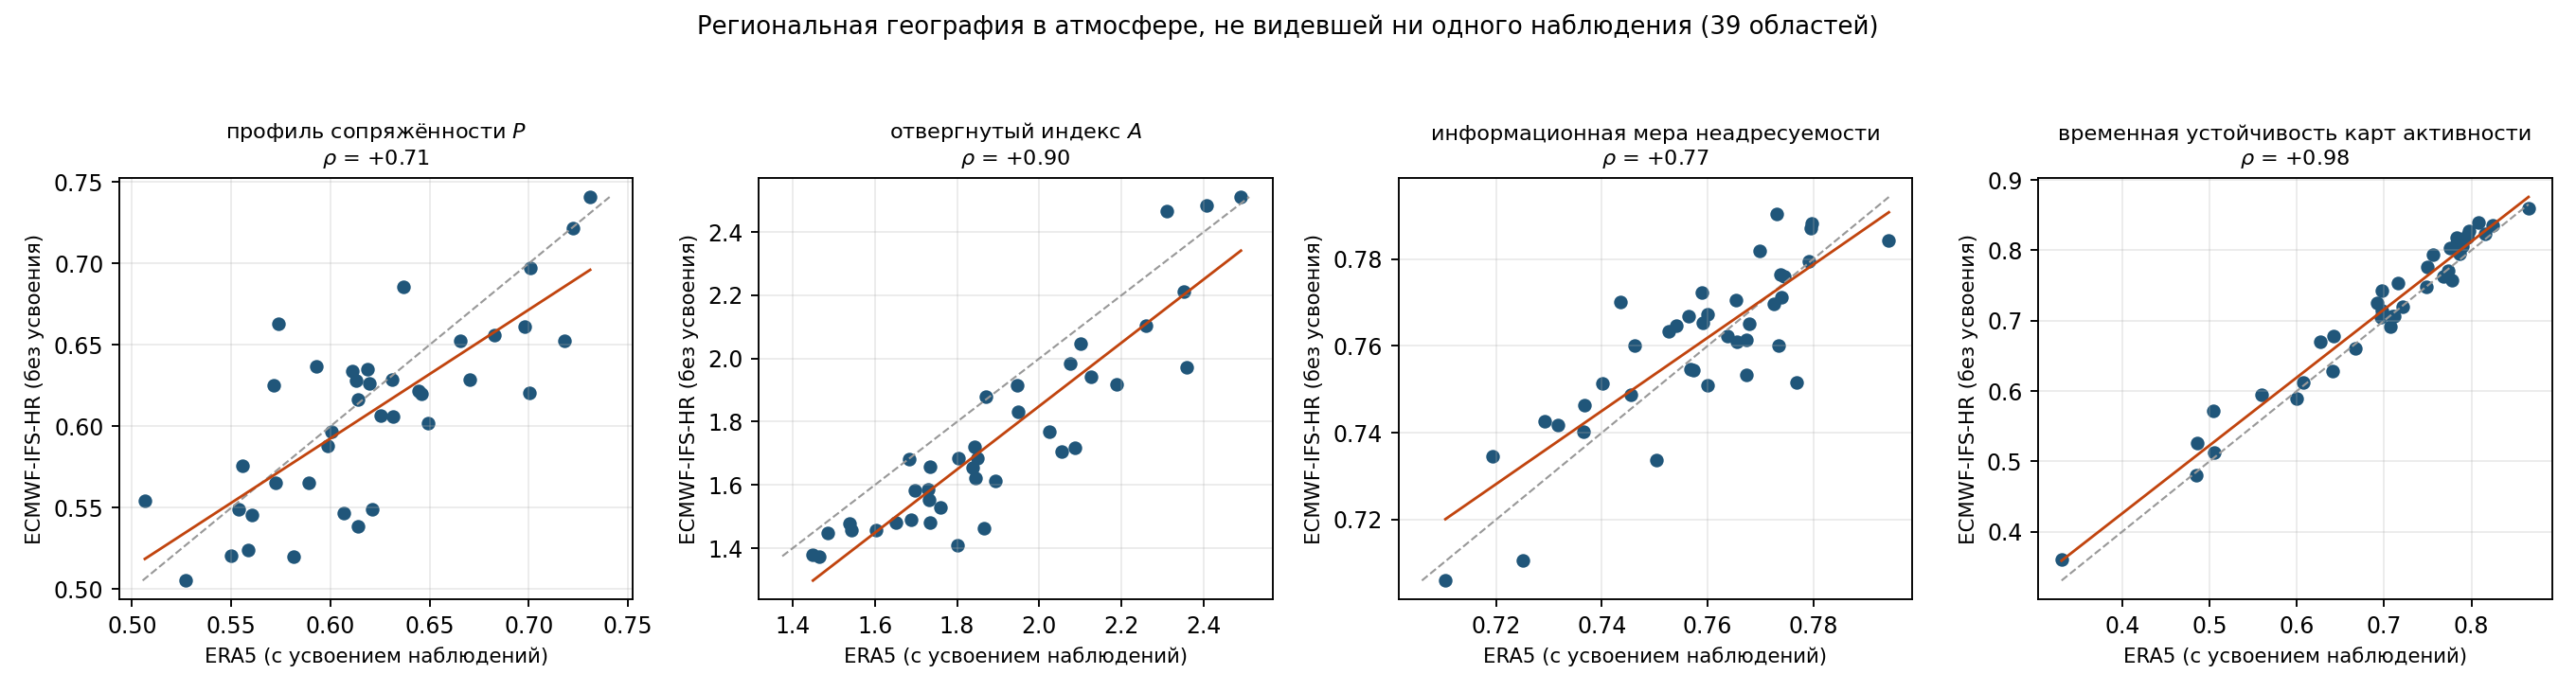
\includegraphics[width=\linewidth]{figures/figP_free_running.png}
\caption{Comparison of the regional geography from ERA5 (abscissa) and from the free-running ECMWF-IFS-HR computation without data assimilation (ordinate) for the 39 domains. Left to right: the coupling profile $P$; the rejected non-reciprocity index $A$; the information measure of non-addressability; the temporal persistence of the activity maps. The dashed line is the identity.}
\label{fig:free}
\end{figure}

\subsection{An independent check of what the quantity measures}

We tested separately whether the profile measures what is ascribed to it. To this end an independent measure was constructed --- the normalized mutual information between the activity maps of adjacent levels, computed on ranks and therefore insensitive to the amplitude of the field. The profile agrees with it with a rank correlation of $-0.93$ (the quantities are opposite in sign by construction), while the connection of the profile with band amplitude is only $+0.20$, and with the temporal persistence of the activity maps $+0.02$.

This is not an external validation: both quantities are statistics of one and the same joint distribution, and a high correlation between them means consistency, not predictive power. But it establishes the main point --- the profile is a faithful summary of precisely the addressability in question, and is a shadow neither of amplitude nor of the inertia of the field.

\subsection{The Congo and the Amazon}

An instructive case is the pair of deep-convection centres over land at similar latitudes. Under a similar moisture regime the Congo and Amazon basins exhibit qualitatively different architectures of the hierarchy (Fig.~\ref{fig:congo}). The difference is concentrated on the top step of the profile: the median over eight seasonal windows is $\rho_5=0.70$ for the Congo against $0.42$ for the Amazon, while on the fine steps the profiles are close (0.89 and 0.84 on the first step).

In substance this means the following. In the Congo basin the centres of mesoscale activity are placed predominantly where the adjacent coarse level is active: the joint distribution of ranks is stretched along the diagonal, and from the large-scale field one can point to where the mesoscale will be. In the Amazon the same pair of levels is distributed almost indifferently: mesoscale organization is to a considerable degree detached from the coarse field. The difference is stable across years and is reproduced on independent periods.

The example shows what matters most for applications: the descriptor discriminates between territories indistinguishable by the standard characteristics of a regime --- by precipitation totals, by convective potential, by the spectrum --- and discriminates them by a feature directly relevant to the problem of generalization. Precisely here lies its immediate use for regionalization.

\begin{figure}[t]
\centering
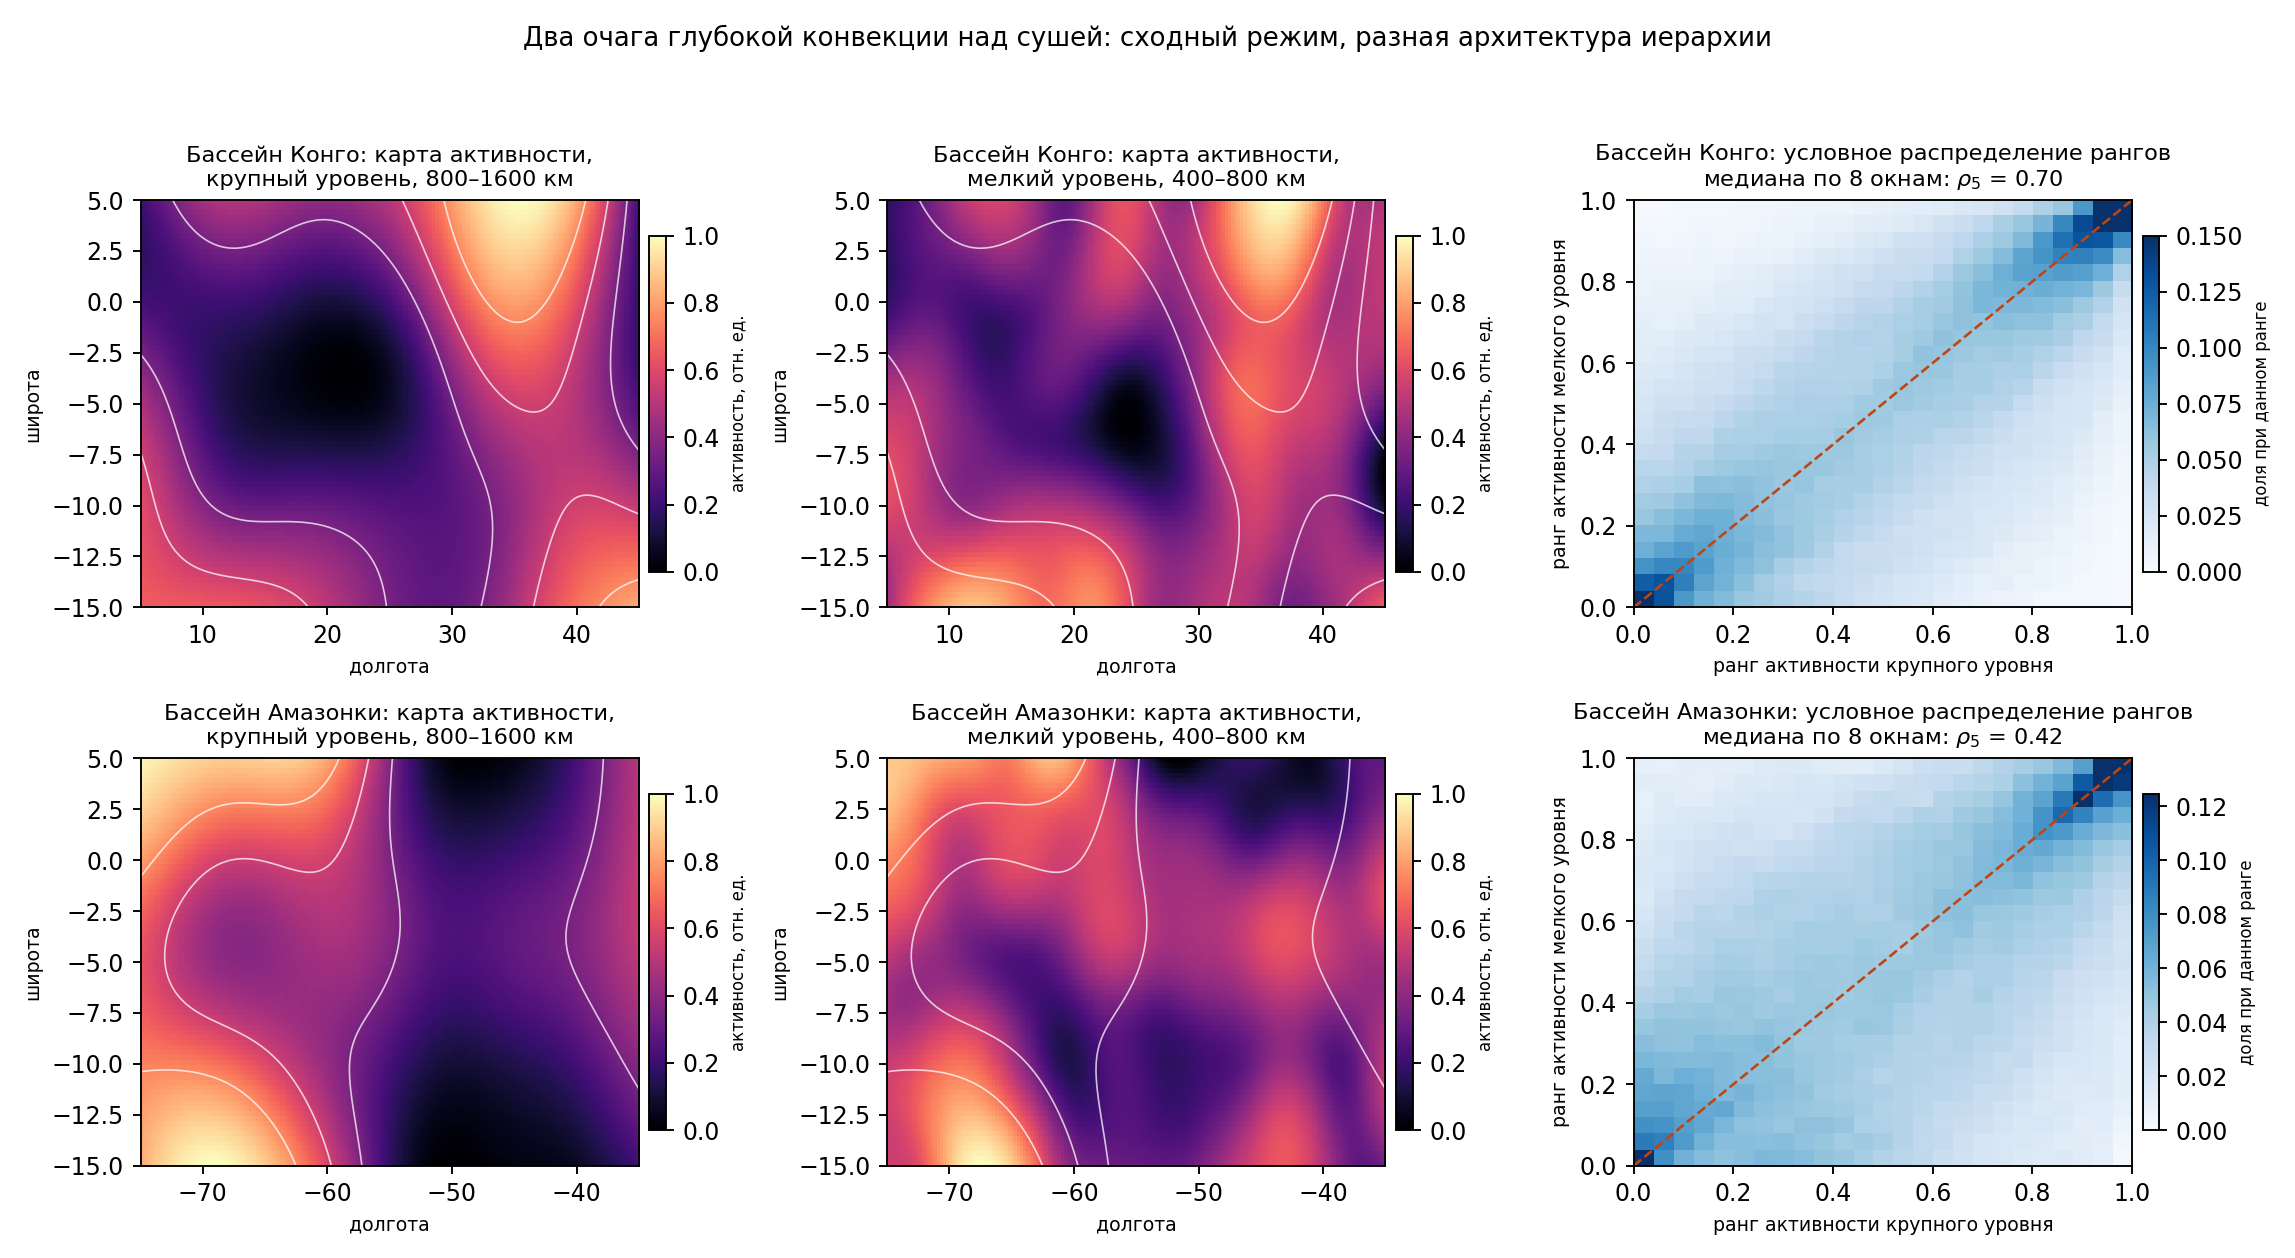
\includegraphics[width=\linewidth]{figures/figP_congo_amazon.png}
\caption{The Congo basin (top) and the Amazon basin (bottom), January--March 2023. Left and centre --- activity maps of the coarse (800--1600~km) and fine (400--800~km) levels at one time step; the white isolines show the activity of the coarse level and are the same on both maps of a row. Right --- the conditional distribution of the spatial ranks of the two levels' activity over all time steps of the window; the dashed line is the diagonal of perfect correspondence. In the Congo the mesoscale activity is tied to the coarse field; in the Amazon it is not.}
\label{fig:congo}
\end{figure}

\section{Tested and rejected interpretations}
\label{sec:limits}

Alongside the confirmed properties, a series of possible readings was tested and rejected. We give them in full (Table~\ref{tab:negative}): they delimit the range of correct use and forestall over-interpretation.

\subsection{The rejected construction of a second descriptor}

Originally a second descriptor was proposed alongside the profile --- a non-reciprocity index $A$, built as a measure of how far the statistical operators of aggregation and refinement fail to commute. It was ascribed the meaning of the irreversibility of geographical generalization: large values were to mean that the placement of the mesoscale cannot be recovered from the large-scale field even statistically.

The index does form a stable regional signature, is reproduced in MERRA-2 with $\rho=0.93$ and in the free-running computation with $\rho=0.90$. But the test of the content of the quantity did not confirm it. On synthetic fields in which the recoverability of the fine level from the coarse one is set by construction and varied systematically, the index does not respond to it either in the spatial reading ($\rho=-0.32$) or in the reading through the predictability of the level coefficients ($\rho=-0.35$), whereas the independent information measure responds correctly ($+0.92$ and $-0.93$ respectively). On the same synthetic fields the index follows the temporal persistence of the field monotonically and strongly ($\rho=1.00$), and this is confirmed on real data: the connection of the index with the persistence of the activity maps is $+0.53$, and with the information measure of non-addressability $+0.03$. More than half of the inter-regional variability of the index is explained linearly by the set of persistence, amplitude, spectral slope and domain geometry.

The conclusion has to be a definite one: the index $A$ is a reproducible regional characteristic of the atmosphere, but a characteristic of the \emph{temporal persistence} of the field, not of the irreversibility of generalization. The reading ascribed to it is rejected; the construction itself is withdrawn from the main exposition. The cause of the error has been established and is methodological: the operators are estimated over a sliding window, and the more slowly the field changes, the more systematically the result is displaced.

\subsection{Other rejected readings}

\emph{The descriptors do not measure the cross-scale flux of kinetic energy.} Direct comparison with the flux computed by spatial coarse-graining \cite{Germano1992,Aluie2018} on a numerical experiment with a known solution explains fractions of a percent of its variability, against $0.35$--$0.47$ for the standard characteristics of the deformation field.

\emph{No simple law connecting the shape of the profiles with environmental covariates was found.} Neither a renormalization of the scale axis, nor the removal of zonal banding, nor the transition to the field of integrated water-vapour transport brings the profiles of different regions onto a single curve.

\emph{No vertical universality was found.} At 500~hPa the regional signature is not statistically confirmed, and the agreement with the 850~hPa geography is insignificant; the sample is half the size of the main one, so the correct statement is an absence of confirmation, not a demonstrated difference.

\emph{The descriptors carry no information about the moisture-budget residual.} The residual of the moisture-budget equation in a reanalysis is governed chiefly by assimilation increments \cite{Trenberth1991,Mayer2021}, and adding inter-level characteristics of the circulation to the standard predictor set does not improve its description.

\emph{There is no instantaneous local connection with precipitation.} At the regime level a stable negative correlation is found, together with a lagged structure with a characteristic time of about two days consistent with the known cycle of the expenditure and recovery of convective energy \cite{Masunaga2012,PetersNeelin2006}; but attempts to formalize this as a dynamical equation failed, and the characteristic time is partly reproduced by the inertia of the estimator itself.

\begin{table}[t]
\centering
\caption{Tested and rejected interpretations.}
\label{tab:negative}
\small
\begin{tabular}{@{}p{0.56\linewidth}p{0.38\linewidth}@{}}
\toprule
Proposition under test & Outcome\\
\midrule
The non-reciprocity index $A$ measures the irreversibility of generalization & rejected (does not respond to controlled recoverability; follows the temporal persistence of the field)\\
The descriptors track the cross-scale flux of kinetic energy & rejected (deformation-field characteristics are two orders of magnitude more informative)\\
The shape of the profiles obeys a universal law in environmental covariates & rejected (no collapse onto a single curve)\\
The descriptors are vertically universal (transfer to 500~hPa) & not confirmed (level specificity)\\
The descriptors are informative for closing the reanalysis moisture budget & rejected\\
The regime-level connection with precipitation can be formalized as a source--sink equation & not established\\
The descriptors predict the growth rate of ensemble forecast error & rejected (see Sect.~\ref{sec:applied})\\
The descriptors predict the level of mesoscale analysis error & rejected (see Sect.~\ref{sec:applied})\\
\bottomrule
\end{tabular}
\end{table}

\section{Applied content: what we are limited by}
\label{sec:applied}

The natural expectation is that a measure of the subordination of the mesoscale to the coarse field should say something about forecast quality and about the justification of statistical downscaling. This expectation was tested in three independent settings, and none was confirmed.

\emph{The growth rate of ensemble forecast error.} Comparison with an operational ensemble system over the 39 domains revealed no connection in the predicted direction; moreover, the regional differences in the error growth rate are governed by baroclinicity --- the correlation with the modulus of latitude is $+0.86$ --- and not by the architecture of the hierarchy.

\emph{The level of mesoscale error at analysis time.} The disagreement of two independent assimilation systems at the mesoscale, taken as a direct measure of placement uncertainty, is connected with the descriptors only through the amplitude of the field: once the controls are removed, the connection disappears.

\emph{The loss of the mesoscale in machine-learning models.} Modern neural weather-prediction models \cite{Lam2023,Bi2023,Price2025} systematically lose mesoscale variability, and the size of the loss admits precise measurement on a common comparison platform \cite{Rasp2024}. At a five-day lead in the 200--800~km band the deterministic models lose 55--69\,\% of the variance, the mean of a generative ensemble 85\,\%, whereas a physical model and an individual realization of the generative ensemble lose essentially nothing. The mechanism is thereby established unambiguously: the losers are those and only those systems that compute a conditional mean. Yet the geography of this loss, too, is predicted better by a simple spectral characteristic than by the proposed descriptors.

The overall outcome is negative, and it should be read literally. We possess data collected by an observing network whose density is itself geographically inhomogeneous, and models which --- in the machine-learning case --- by the design of their loss functions destroy precisely the mesoscale structure at issue. Under these conditions the absence of a detected connection permits no conclusion either way about the existence of applied content in the measured quantity. It permits a different conclusion: on today's data and today's models such content is not detectable, and a simple spectral characteristic proves the stronger predictor in all three settings. Further progress requires not more statistical tests on the same material but different observations --- above all, homogeneous in density --- and models that preserve mesoscale variability.

\section{Conclusions}
\label{sec:conclusion}

1.~A compact descriptor of the inter-level organization of the atmospheric circulation is proposed --- the octave-level coupling profile $P$, characterizing the degree to which the placement of mesoscale variability is predetermined by the adjacent coarse level.

2.~The descriptor forms a stable regional signature that persists across seasons, years and ENSO phases ($p=0.001$ on samples that took no part in its construction) and is not reducible to the semi-fractal characteristics of the levels or to symmetric statistics of cross-scale coupling. Its independence from the full power spectrum is conditional: it does not survive the additional control of domain geometry.

3.~The regional geography of the descriptor is reproduced not only in an independent reanalysis but also in a model computation that assimilates no atmospheric observations ($\rho=0.71$ against an internal ceiling of the method of $0.93$). The measured property belongs to the atmosphere, not to the observing network and not to the assimilation system. An independent information measure confirms that the descriptor measures precisely addressability, and is a shadow neither of amplitude nor of the inertia of the field.

4.~The greatest coupling belongs to the extratropical storm tracks, the smallest to the moist-convective oceanic regimes; the Congo and Amazon basins, under a similar regime, exhibit qualitatively different architectures of the hierarchy. The characteristic obtained satisfies the operational definition of an invariant of geosystem dynamics and continues the line of research into hierarchical organization --- from the identification of levels to the measurement of their interaction.

5.~The applied content of the quantity has not been established on the data and models available today. Three derived predictions --- on the growth rate of forecast error, on the level of mesoscale analysis error, and on the loss of the mesoscale in machine-learning models --- were tested and not confirmed, a simple spectral characteristic proving the stronger predictor in all three cases. The negative result is reproducible and marks out the direction of further work: observations homogeneous in density, and models that preserve mesoscale variability, are required.

6.~The second descriptor originally proposed --- the index of the non-reciprocity of the aggregation and refinement operators --- retains the status of a reproducible regional characteristic, but the reading ascribed to it as a measure of the irreversibility of generalization is rejected by a direct test: the quantity follows the temporal persistence of the field, not the recoverability of the mesoscale.

\paragraph{Data and code.} The testing protocols with criteria fixed in advance, the program code, the full table of the experiments performed and the numerical results are openly available in the repository: \url{https://github.com/Theclimateguy/Shroedinger}.

\printbibliography[title={References}]

\end{document}
